\section{BPR}

	
\subsection*{Pairwise Preference Assumption}
\begin{frame}
	\frametitle{Pairwise Preference Assumption}
	\begin{columns}
		\column{.6\textwidth}
			\begin{figure}
				\vspace{-7em}
				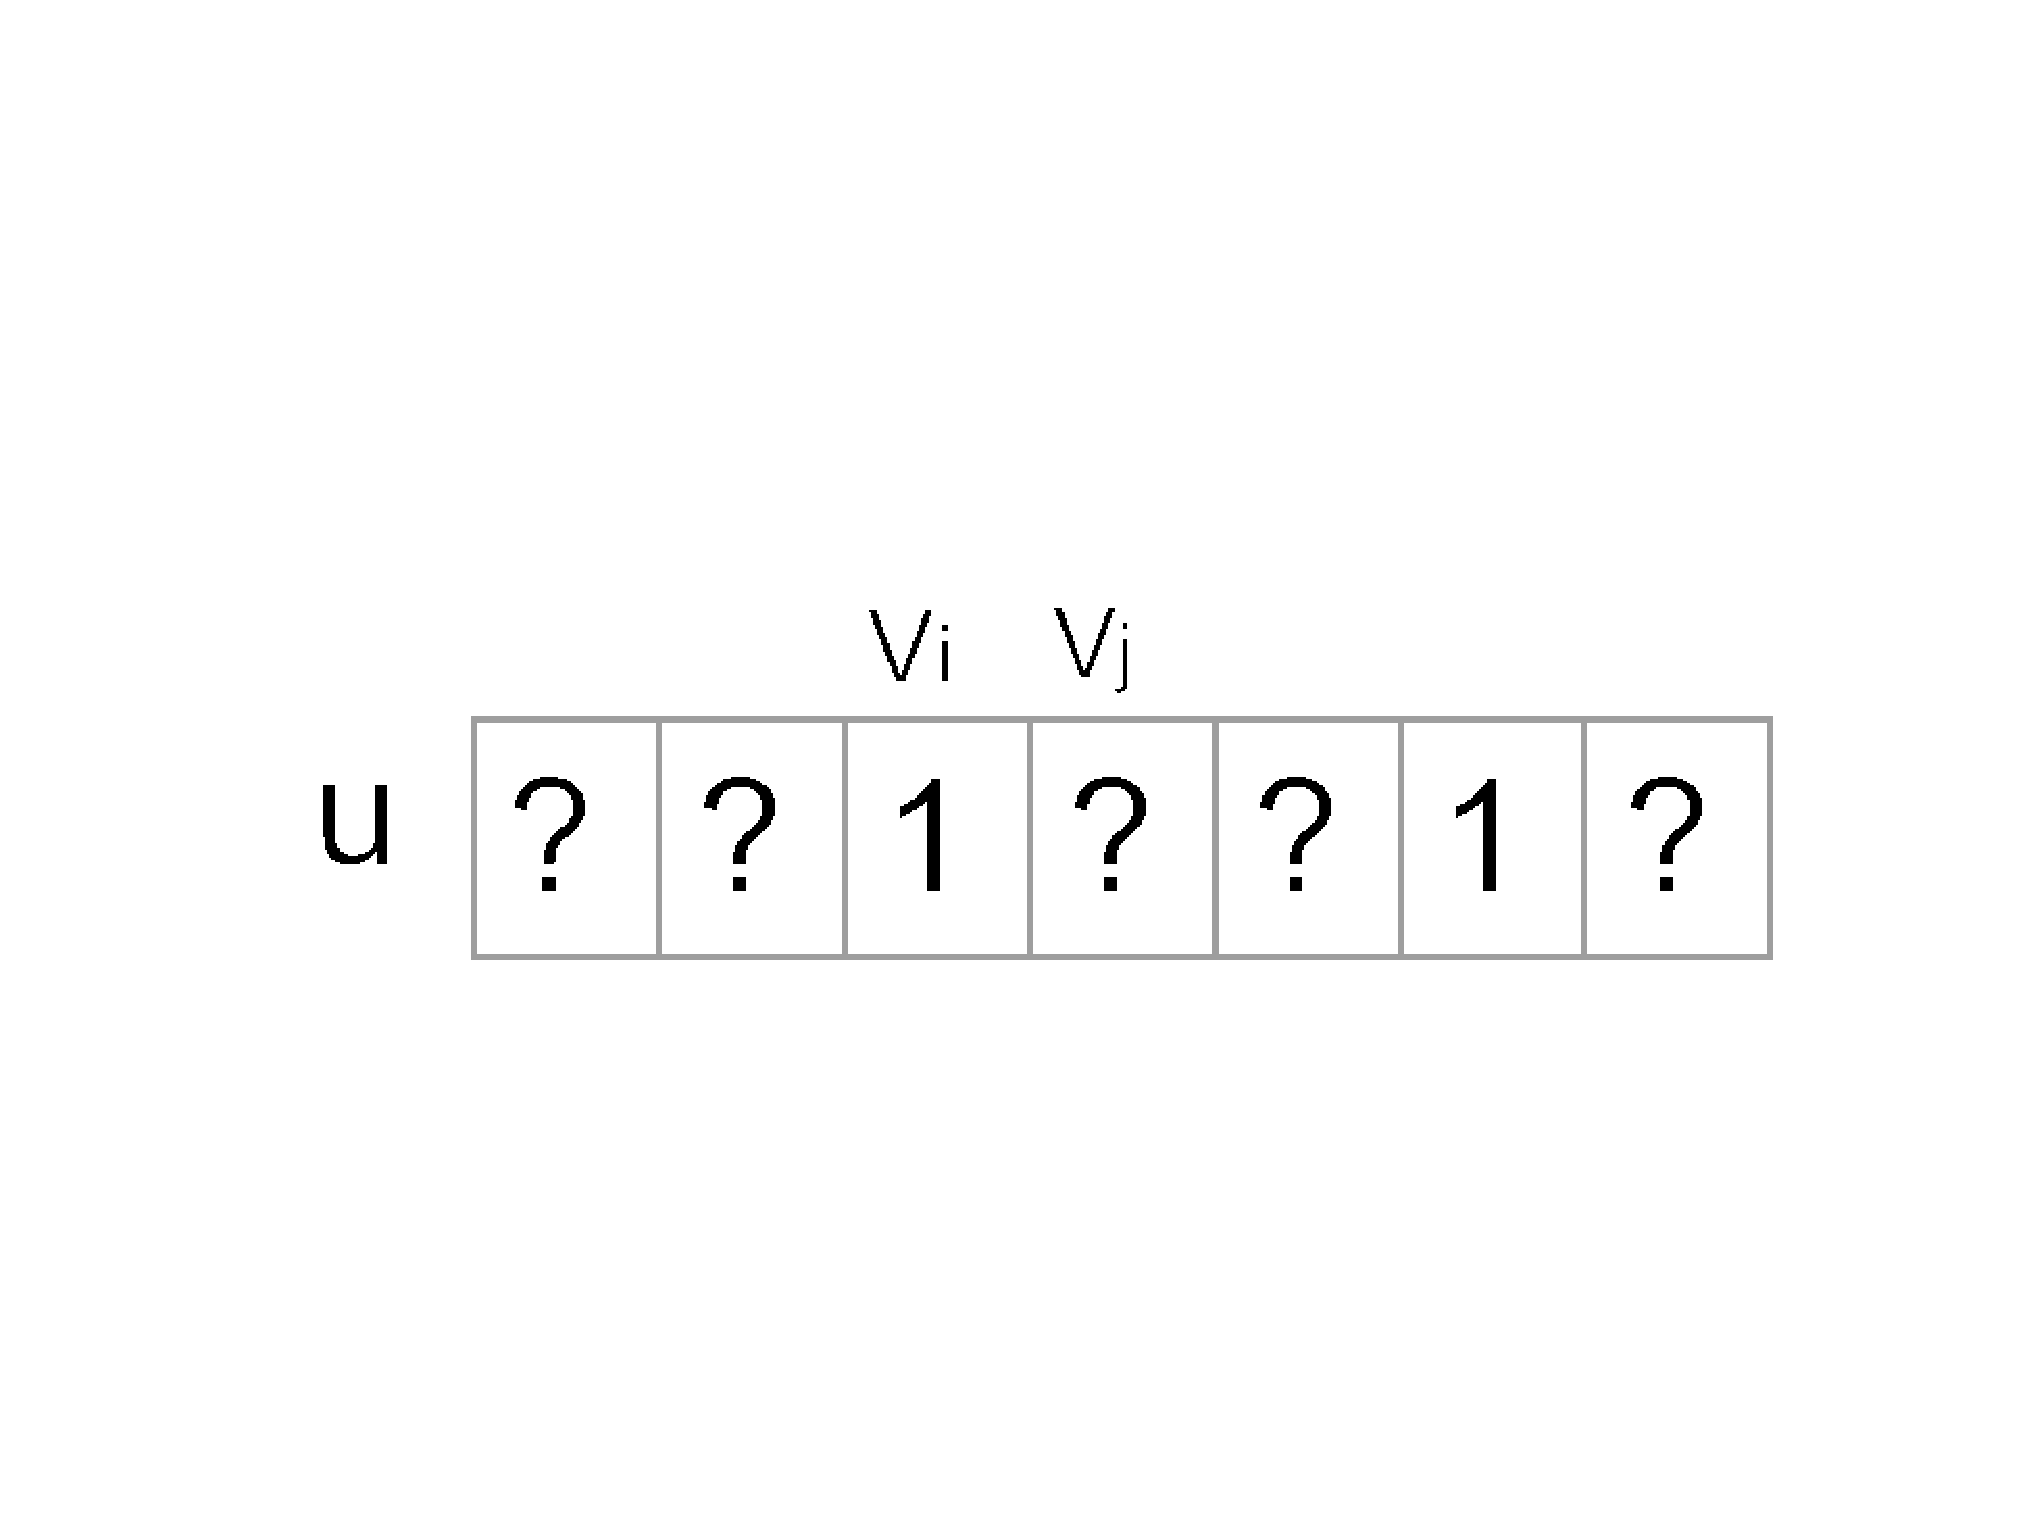
\includegraphics[width=3in]{pairwise}
			\end{figure}
			\vspace{-6em}
			\hspace{4em} \textcolor{red}{user $u$ prefers item $v_i$ over  $v_j$}
			
		\column{.5\textwidth}
		\begin{itemize}
			\item define the pairwise preference of user $u$ as:
			\begin{equation}
			p \left( i \succ_u j \right) := f \left( x_{uij} \right),
			\end{equation}
			where $f \left(x\right) = 1/\left(1+exp\left(-x\right)\right)$, $x_{uij} := \hat{r}_{uij} = \hat{r}_{ui} -\hat{r}_{uj}$.
		\end{itemize}
		
	\end{columns}
\end{frame}

\subsection*{Prediction Rule}
\begin{frame}{Prediction Rule}
	\begin{itemize}
		\vspace{2em}
		\item The predicted rating $\hat{r}_{ui}$ of user $u$ on item $i$ :
		\begin{equation}
		\hat{r}_{ui} = U_{u\cdot}V_{i\cdot}^T + b_i
		\end{equation}
		\begin{centering}
			\begin{figure}
				\vspace{-7em}
				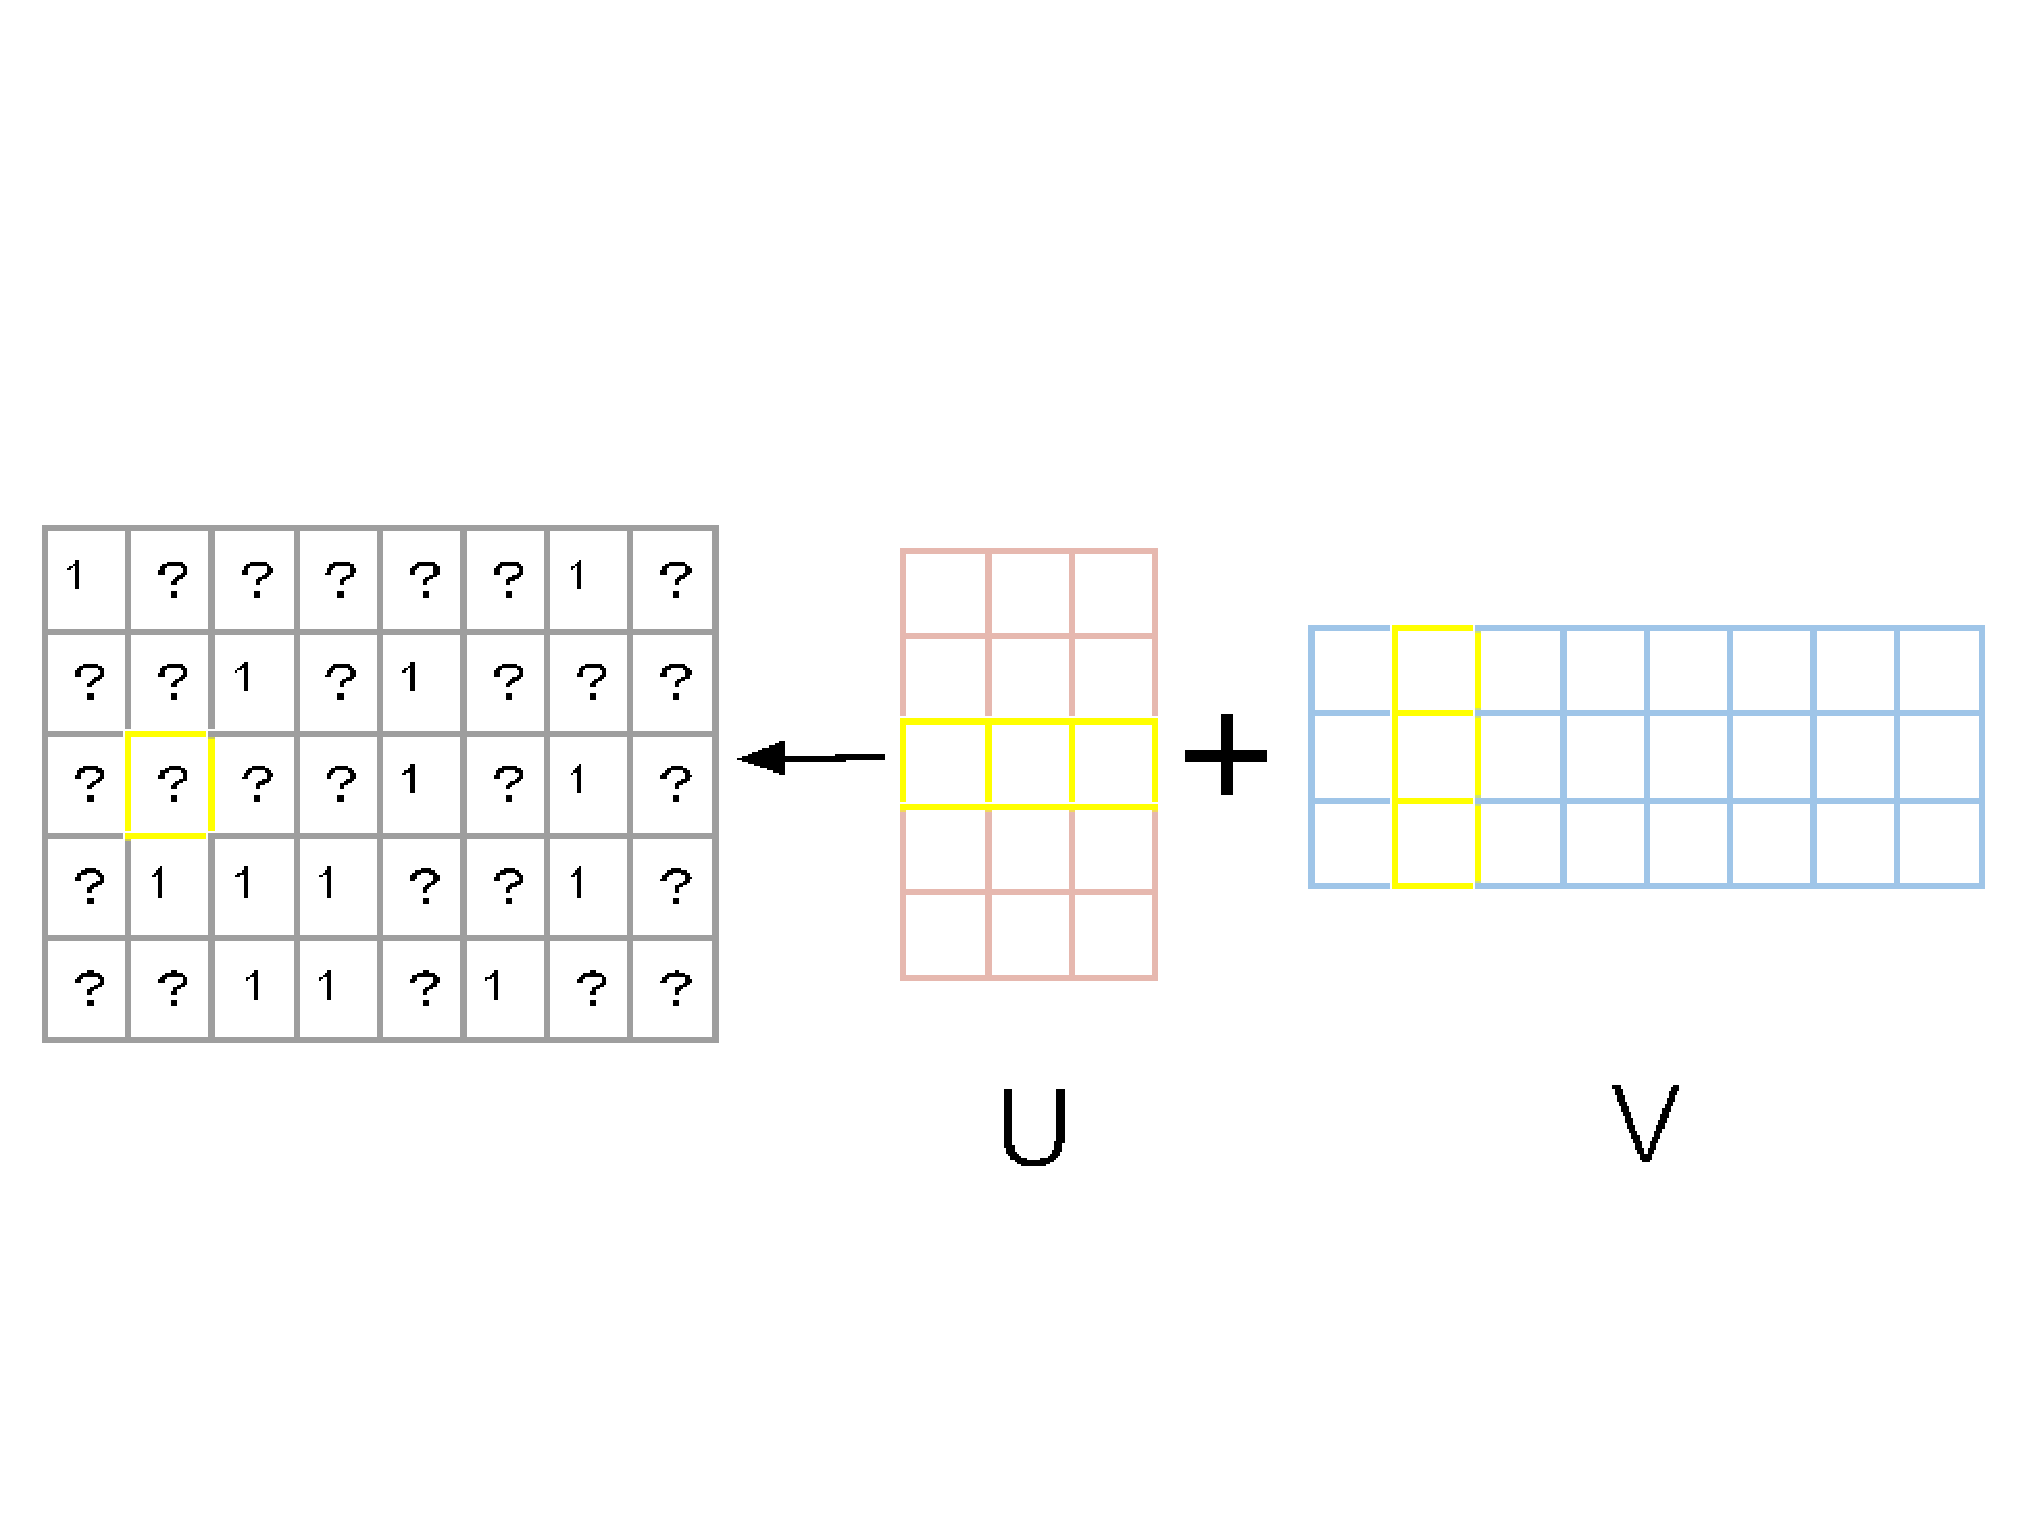
\includegraphics[width=4in]{uv}
			\end{figure}
		\end{centering}
	\end{itemize}
	
\end{frame}


\subsection*{Likelihood of Pairwise Preference}
\begin{frame}{Likelihood of Pairwise Preference}
	\begin{itemize}
		
		\setlength{\itemsep}{2ex plus0.2ex}
		
		\item The random variable $x$ with Bernoulli distribution :
		
		\scalebox{0.8}{
			\parbox{1.2\textwidth}{
				\begin{equation}
				Ber\left(x|p \right)=p^x\left(1-p \right)^{1-x} \qquad  \text{for}\  x \in \{0,1\},p \in [0,1]
				\end{equation}
			}
		}
		
		
		\item The Bernoulli distribution of binary random variable $x \left(\left(u,i\right) \succ \left(u,j\right)\right)$ is
		defined as follows :
		%%%%公式太长了先放入到一个盒子中parbox,在对盒子进行缩放scalebox
		\scalebox{0.8}{
			\parbox{1.2\textwidth}{
					\begin{equation}
					\label{eq4}
					\begin{aligned}
					LPP_u  
					&= \prod_{ \ i,j \  \in \  \mathcal{I}}p\left(\hat{r}_{ui} > \hat{r}_{uj}\right)^{x \left(\left(u,i\right) \succ \left(u,j\right)\right)} \left[1-p\left(\hat{r}_{ui} > \hat{r}_{uj}\right)\right]^{1-x \left(\left(u,i\right) \succ \left(u,j\right)\right)}\\
					&= \prod_{\left(u,i\right) \succ \left(u,j\right)}p\left(\hat{r}_{ui} > \hat{r}_{uj}\right)\prod_{\left(u,i\right) \preceq \left(u,j\right)}\left[1-p\left(\hat{r}_{ui} > \hat{r}_{uj}\right)\right]
					\end{aligned}
					\end{equation}
				}
		}
		where \textcolor{red}{$(u,i) \succ (u,j)$ means that user $u$ prefers item $i$ to item $j$}.
	\end{itemize}
\end{frame}




\subsection*{Objective Function}
\begin{frame}{Ojective Function}
	\begin{itemize}
		\item  Given a set of pairwise preference $D_S$ , the
		goal of BPR is to maximize the likelihood of all pairwise
		preference:
		\begin{equation}
		arg \ \max_{\substack \Theta } \prod_{\left(u,i,j\right) \in D_S} p\left(i \succ_u j\right),
		\end{equation}
		which is equivalent to minimize the negative log likelihood:
		\begin{equation}
		\label{eqbprojc}
		L_{feedback} = - \sum_{\left(u,i,j\right) \in D_S}\ln f \left( \hat{r}_{uij}\right) + \lambda\|\Theta\|^2,
		\end{equation}
		where $\hat{r}_{uij} = \hat{r}_{ui} - \hat{r}_{uj}$, $\Theta$ denotes the set of all latent vectors and $\lambda$ is a hyper-parameter.
	\end{itemize}
\end{frame}

\begin{frame}{Ojective Function}
	\begin{itemize}
		\item Specifically, Eq\eqref{eqbprojc} is to minimize the following objective function  : 
		\begin{equation}
		\min_{\substack\Theta}\sum_{u\in\mathcal{U}}\ \sum_{i\in\mathcal{I}_u}\sum_{j\in\mathcal{I}\setminus\mathcal{I}_u}\Phi_{uij}
		\end{equation}
		where
		$\Phi_{uij}
		= 
		- \ln f \left(\hat{r}_{uij}\right) 
		+ \frac{\alpha_u}{2}\|U_{u\cdot}\|^2
		+ \frac{\alpha_v}{2}\|V_{i\cdot}\|^2
		+ \frac{\alpha_v}{2}\|V_{j\cdot}\|^2
		+ \frac{\beta_v}{2}\|b_{i}\|^2
		+ \frac{\beta_v}{2}\|b_{j}\|^2$, $\Theta = \{U_{u\cdot},V_{i\cdot},b_i\}
		$ denotes the parameters to learn.
	\end{itemize}
\end{frame}



\subsection*{SGD}
\begin{frame}{SGD}
	\begin{itemize}
		
		\setlength{\itemindent}{-2ex}
		
		\item For a randomly sampled triple $\left(u,i,j\right)$, calculate the partial derivative for $U_{u\cdot}$:
		
		\vspace{3ex}
		
		\scalebox{0.8}{
			\parbox{1.2\textwidth}{
				\begin{equation}
				\hspace{-9ex}
				\begin{aligned}
				\bigtriangledown U_{u\cdot} 
				= \frac{\partial \Phi_{uij}}{\partial U_{u\cdot}}
				&=-\frac{\partial \ln f\left(\hat{r}_{uij}\right)}{\partial f\left(\hat{r}_{uij}\right)} 
				\frac{\partial f\left(\hat{r}_{uij}\right) }{\partial \hat{r}_{uij}} 
				\frac{\partial \hat{r}_{uij}}{\partial U_{u\cdot}}
				\ + \  \alpha_uU_{u\cdot}\\
				&= -\frac{1}{f\left(\hat{r}_{uij}\right)} 
				\frac{\partial f\left(\hat{r}_{uij}\right) }{\partial \hat{r}_{uij}} 
				\frac{\partial \hat{r}_{uij}}{\partial U_{u\cdot}}
				\ + \  \alpha_uU_{u\cdot}\\
				&= -\frac{1}{f\left(\hat{r}_{uij}\right)} 
				{f\left(\hat{r}_{uij}\right) f\left(-\hat{r}_{uij}\right)}
				\frac{\partial f\left(\hat{r}_{ui} - \hat{r}_{uj}\right) }{\partial U_{u\cdot}} 
				\ + \ \alpha_uU_{u\cdot}\\
				&= -{f\left(-\hat{r}_{uij}\right)} \frac{\partial f\left[\left(U_{u\cdot}V_{i\cdot}^T+b_i\right) - \left(U_{u\cdot}V_{j\cdot}^T+b_j\right)\right] }{\partial U_{u\cdot}} 
				\ + \ \alpha_uU_{u\cdot}\\
				&= -{f\left(-\hat{r}_{uij}\right)} \left(V_{i\cdot} - V_{j\cdot}\right)  
				\ + \  \alpha_uU_{u\cdot}\\
				\end{aligned}
				\end{equation}
			}
		}
	\end{itemize}
\end{frame}
\begin{frame}{SGD}
	\begin{itemize}
		\item For the rest of parameters, we have the partial derivatives:
		\begin{align} %align环境不要有空行
		\bigtriangledown V_{i\cdot} &= \frac{\partial \Phi_{uij}}{\partial V_{i\cdot}}=-f\left(-\hat{r}_{uij}\right)U_{u\cdot} + \alpha_vV_{i\cdot}\\
		\bigtriangledown V_{j\cdot} &= \frac{\partial \Phi_{uij}}{\partial V_{j\cdot}}=-f\left(-\hat{r}_{uij}\right)\left(-U_{u\cdot}\right) + \alpha_vV_{j\cdot}\\
		\bigtriangledown b_i        &= \frac{\partial \Phi_{uij}}{\partial b_i} =-f\left(-\hat{r}_{uij}\right)+\beta_vb_i\\
		\bigtriangledown b_j        &= \frac{\partial \Phi_{uij}}{\partial b_j} =-f\left(-\hat{r}_{uij}\right)\left(-1\right)+\beta_vb_j
		\end{align}
		where $ \hat{r}_{uij} = \hat{r}_{ui} - \hat{r}_{uj}$. 
	\end{itemize}
\end{frame}
\begin{frame}{Update Rules}
	\begin{itemize}
		\item For a randomly sampled triple $(u,i,j)$, we have the update rules,
		\begin{align}
		\label{eq10}
		U_{u\cdot} &= U_{u\cdot} - \gamma\bigtriangledown U_{u\cdot}\\
		V_{i\cdot} &= V_{i\cdot} - \gamma\bigtriangledown V_{i\cdot}\\
		V_{j\cdot} &= V_{i\cdot} - \gamma\bigtriangledown V_{j\cdot}\\
		b_{i\cdot} &= b_i - \gamma\bigtriangledown b_{i}\\
		b_{j\cdot} &= b_j - \gamma\bigtriangledown b_{j}
		\end{align}
		where $\gamma$ is the learning rate.
	\end{itemize}
\end{frame}

\subsection*{SGD for BPR}
\begin{frame}{The SGD algorithm for BPR}
	\IncMargin{1em}%将行号对齐到里面
	\begin{algorithm}[H]%beamer中使用算法,需要[H]选项否则会出现outer mode错误
		\SetAlgoNoLine %不要算法中的竖线
		\BlankLine
		
		initialize the model parameter $\Theta$\;
		\For {$t_1 = 1,\cdots,T$}{
			\For {$t_2 = 1,\cdots, |\mathcal{P}|$}{
				Randomly pick up a pair $\left(u,v_i\right) \in \mathcal{P}$\;
				{\color{red}{Randomly pick up an item $v_j$ from $\mathcal{I} \setminus \mathcal{I}_{u}^+$}\;}
				Calculate the gradients via Eq.(8-12)\;
				Update the model parameters via Eq.(13-17)\;
			}	
		}
		\caption{The SGD algorithm for BPR}
		\label{al1}%label 放置的位置有讲究, 放后面
	\end{algorithm}
	\DecMargin{1em}
	
\end{frame}

